% !TeX spellcheck = en_GB
\chapter{Methodological Approach} \label{chap:method-approach}

In this chapter, we will formally state the problem this work aims to address, as well as its the proposed solution. In section \ref{sec:problem} the problem statement is exposed, section \ref{sec:requirements} lists the solutions main functional, non-functional and structural requirements, section \ref{sec:arch} addresses the architecture of the solution, section \ref{sec:method} exposes the established methodology and section \ref{sec:work-plan} contains the proposed work plan.

\section{Problem Statement} \label{sec:problem}

\begin{displayquote}
	 \textit{The reviewed literature addressing solutions to sequential decision-making problems in graph-based environments is sparse and scarce, leading to a research gap for comparative and systematic \ac{GRL} approaches analysing scalability under different sized scenarios and adaptability to topology variation.}
\end{displayquote}

As addressed in the previous chapter, graphs are ubiquitous representations that can serve to instinctively represent several problems and their objects. In some network-oriented domains, these representations reveal underlying features that can't be naturally represented by plain Euclidean data. This problem becomes even more difficult considering that graph data is complex and sparse, something that brings the need for methods that efficiently extract representations. \par
By conducting a thorough literature review of the relevant studies in this context, we observed that current \ac{RL} algorithms are not as efficient as \ac{GRL} techniques in handling such complex environments, because of not considering and generalizing environment topology features in the decision-making process. This deeply affects the performance of decision systems inserted in network-oriented domains where the intricate relationships between the objects may be relevant for mapping the observable environment states to optimal action policies. \par
More and more \ac{GRL} attracts the curiosity of academics, only increasing the relevance of this problem. With the recent advancements of \acp{GNN}, the popularity around \ac{GRL} has risen because of their excellent efficiency in creating optimal graph representations and other graph machine learning problems. However, with \ac{GRL} being a field whose research is still in initial phase, the gathered literature is very sparse, with a lack of works addressing the benefits, disadvantages and performance of the various proposed models. Moreover, the literature also highlights the importance of studying \ac{GRL} models in scenarios under topology variations and of different sizes for analysing their scalability. \par

\subsection{Scope}

This dissertation will focus on studying this problem in the context of single-agent \ac{RL} algorithms, given that multi-agent systems are significantly more complex to implement. Furthermore, in the context of the dissertation's application domain, which is smart grid services, the possible improvements in \ac{GRL} techniques will be implemented to the \acf{DED} problem that studies solutions that optimize power generation cost while maintaining reliable grid stability. Additionally, the \ac{GRL} proposed models may be also implemented to solve other smart grid systems such as Undervoltage Load Shedding and Volt-VAR Regulation.

\section{Problem Formalization}

In this section, the main problem of study of this dissertation is formally introduced. Firstly, the problem is approached from an application domain perspective, uncovering the details of the \ac{DED} problem and its main features. In the sequent subsection, the \ac{DED} problem is formalized as a dynamic sequential decision-making problem, and its characteristics are presented under the form of its corresponding \ac{MDP}.

\subsection{Dynamic Economic Dispatch}

\begin{comment}
	* Citation Needed (?)
	* Revise
	* Constraints
	
	
	
	
	
	
	
\end{comment}

\begin{center}
	\begin{tabular}{ | m{2cm} | m{10cm}| } 
		\hline
		$F(t)$ & Total Operational Cost \\ 
		\hline
		$F_\text{NRES}(t)$ & Total Non-Renewable Generators Operational Cost \\
		\hline
		$F_\text{NRES}(t)$ & Total Renewable Generators Operational Cost \\
		\hline
		$F_\text{ESS}(t)$ & Total ESS Operational Cost \\
		\hline
		$T$ & Terminal Timestep \\
		\hline
		$t$ & Timestep \\
		\hline
		$c^\text{NRES}_i$ & Cost of conventinal generator $i$ in €/MWh \\
		\hline
		$P^\text{NRES}_i(t)$ & Current generated power of non-renewable generator $i$ in MW \\
		\hline
		$\beta_\text{RES}$ & \ac{RES} wasted energy penalty term \\
		\hline
		$P^\text{RES}_i(t)$ & Current generated power of renewable generator $i$ in MW \\
		\hline
		$\overline{P^\text{RES}_i}(t)$ &  Current power of renewable generator $i$ before curtailmentin MW \\
		\hline
		$c^\text{ESS}_i$ & Operational Cost of \ac{ESS} $i$ in €/MW \\
		\hline
		$P^\text{ESS}_i(t)$ & Discharging/Charging Power of \ac{ESS} $i$ \\
		\hline
		$P^\text{LOAD}_i(t)$ & Active Power demand of load $i$ \\
		\hline
		$Q^\text{LOAD}_i(t)$ & Reactive Power demand of load $i$ \\
		\hline
		$F_i$ or $F_{i,j}$ & Powerline $i$ status \\
		\hline
		$\text{rho}_i$ or $\text{rho}_{i,j}$ & Relative flows of powerline $i$ or with origin in substation $i$ and destination in substation $j$. Ratio of the flow divided by its thermal limit. \\
		\hline
		$P^\text{G}_i(t)$ & Current generated active power of generator $i$ in MW \\
		\hline
		$Q^\text{G}_i(t)$ & Current generated reactive power of generator $i$ in MW \\
		\hline
		$N$ & Number of non-renewable generators \\
		\hline
		$M$ & Number of renewable generators \\
		\hline
		$K$ & Number of loads \\
		\hline
		$L$ & Number of powerlines \\
		\hline
	\end{tabular}
\end{center}

\subsubsection{Objective Function}

The \ac{DED} problem addresses the issue of balancing the necessity for ensuring stability, security and reliability of a power grid while also minimizing its operating cost. This problem is hardened by the paradigm observed in current power systems where \ac{ESS} and \ac{RES} are available and also need to be taken in consideration when studying solutions for this problem. \par
Equation \ref{eq:ded-function} highlights the main objective function for the \ac{DED} problem and is composed of three main components: $F_\text{NRES}(t)$ represents the cost of energy produced by conventional generators, $F_\text{RES}(t)$ is the term that depicts the cost of wasted energy from \ac{RES} and $F_{\text{ESS}}(t)$ the \ac{ESS} operation cost. \par

\begin{equation} \label{eq:ded-function}
 \min\sum^T_{t=1}F_\text{NRES}(t) + F_{\text{RES}}(t) + F_{\text{ESS}}(t)
\end{equation}

Conventional generation cost calculation is presented in equation \ref{eq:conv-cost}. For the sake of simplicity, this component is reduced to a linear equation and represented by a static $c_i$ term for generator $i$ in €/MWh . Regarding the cost of wasted \ac{RES} energy, a penalty term $\beta_\text{RES}$ is introduced that defines a cost for the abandoned renewable energy. Lastly, concerning \acp{ESS}, the cost is directly related to its operation cost $c^\text{ESS}_i$ in €/MW and to its current discharging/charging power $P^\text{ESS}_i$ with a positive power meaning that energy is being absorbed.

\begin{equation} \label{eq:conv-cost}
	F_\text{NRES}(t) = \sum^N_{i=0} c^\text{NRES}_i P^\text{NRES}_i(t) \Delta t
\end{equation}

\begin{equation} \label{eq:res-cost}
	F_\text{RES}(t) = \beta_\text{RES} \sum^M_{i=0}  (\overline{P^\text{RES}_i}(t) - P^\text{RES}_i(t)) \Delta t 
\end{equation}

\begin{equation} \label{eq:ess-cost}
	F_\text{ESS}(t) = \sum^O_{i=0} c^\text{ESS}_i P^\text{ESS}_i(t) 
\end{equation}


\subsubsection{Constraints}


\subsection{\acf{MDP}}



\begin{comment}
	* Voltage Deviation
\end{comment}

In this section, the \ac{DED} problem is formalized in the as a sequential decision-making problem and its \ac{MDP} is uncovered. 

\subsubsection{Simple}

\begin{description}
	\item[Action] The considered action space includes the change in conventional generator redispatching $\Delta P^G_i$, renewable energy curtailment $P^\text{RES}_i$ and \ac{ESS} absorption/production power $P^\text{ESS}_i$.
	
	\item[Observation] The observation space is composed of four components regarding Generators, \ac{RES}, Loads and Powerlines, highlighted in the following equations:
	
	\begin{comment}
		* Voltage
	\end{comment}
	
	\begin{equation} \label{eq:simple-obs-space1}
		o_{1}(t)= \begin{bmatrix}
			P^\text{NRES}_1 & P^\text{NRES}_2 & \dots & P^\text{NRES}_{N} \\
		\end{bmatrix}
	\end{equation}
	
	\begin{equation} \label{eq:simple-obs-space2}
		o_{2}(t)= \begin{bmatrix}
			P^\text{RES}_1 & P^\text{RES}_2 & \dots & P^\text{RES}_{M} \\
			\overline{P^\text{RES}_1} & \overline{P^\text{RES}_2} & \dots & \overline{P^\text{RES}_{M}} \\
		\end{bmatrix}
	\end{equation}
	
	\begin{equation} \label{eq:simple-obs-space3}
		o_{3}(t)= \begin{bmatrix}
			P^\text{LOAD}_1 & P^\text{LOAD}_2 & \dots & P^\text{LOAD}_{K} \\
			Q^\text{LOAD}_1 & Q^\text{LOAD}_2 & \dots & Q^\text{LOAD}_{K} \\
		\end{bmatrix}
	\end{equation}
	
	\begin{equation} \label{eq:simple-obs-space4}
		o_{4}(t)= \begin{bmatrix}
			F_1 & F_2 & \dots & F_{L} \\
			\text{rho}_1 & \text{rho}_2 & \dots & \text{rho}_{L} \\
		\end{bmatrix}
	\end{equation}
	
	\begin{equation} \label{eq:simple-obs-space}
		o(t)= \{ o_{1}(t), o_{2}(t), o_{3}(t), o_{4}(t) \}
	\end{equation}
	
	This tuple encompasses the main elements of the powergrid an their characteristics, without capturing their topology.
	
	\item[Reward] 
	
	\begin{equation}
		r(t) = r_1(t) + r_2(t)
	\end{equation}
	
	\begin{equation}
		\begin{split}
			r_1(t) &= \overline{F_\text{NRES}} - F_\text{NRES}(t) \\
			&= \overline{F_\text{NRES}} - \sum^N_{i=0} c^\text{NRES}_i P^\text{NRES}_i(t) \Delta t
		\end{split}
	\end{equation}
	
	\begin{equation}
		\begin{split}
			r_2(t) &= - F_\text{RES}(t) \\
			&= \beta_\text{RES} \sum^M_{i=0} (\overline{P^\text{RES}_i}(t) - P^\text{RES}_i(t)) \Delta t
		\end{split}
	\end{equation}
\end{description}


\subsubsection{Graph}

\begin{description}
	\item[Action] The considered action space includes the change in conventional generator redispatching $\Delta P^G_i$, renewable energy curtailment $P^\text{RES}_i$ and \ac{ESS} absorption/production power $P^\text{ESS}_i$.
	
	\item[Observation] The observation space includes the current active and reactive load power, conventional and \ac{RES} generator active power, \ac{RES} power before curtailment, state-of-charge of \ac{ESS} and the current timestep for each node of the grid, respectively represented as a tuple in equation \ref{eq:graph-obs-space}.
	
	\begin{equation} \label{eq:graph-obs-space}
		o_i(t) = \{P^\text{LOAD}_i, Q^\text{LOAD}_i, P^\text{NRES}_i, P^\text{RES}_i, \overline{P^\text{RES}_i}, t\}
	\end{equation}
	
	Beyond that, the observation also includes the topology of the power grid as a graph structure, considering the current powerline status as edges connecting substations and their respective relative flow as their weights. In this manner, the full observation is represented as:
	
	\begin{equation}
		o(t) = G(\text{Adj}, W, X)
	\end{equation}
	
	where 
	
	\begin{equation}
		\text{Adj}_{i,j} = F_{i,j}
	\end{equation}
	
	\begin{equation}
		W_{i,j} = \text{rho}_{i,j}
	\end{equation}
	
	\begin{equation}
		X_i = o_i
	\end{equation}
	
	\item[Reward] description
	
	\begin{equation}
		r(t) = r_1(t) + r_2(t)
	\end{equation}
	
	\begin{equation}
		\begin{split}
			r_1(t) &= \overline{F_\text{NRES}} - F_\text{NRES}(t) \\
			&= \overline{F_\text{NRES}} - \sum^N_{i=0} c^\text{NRES}_i P^\text{NRES}_i(t) \Delta t
		\end{split}
	\end{equation}
	
	\begin{equation}
		\begin{split}
			r_2(t) &= - F_\text{RES}(t) \\
			&= \beta_\text{RES} \sum^M_{i=0} (\overline{P^\text{RES}_i}(t) - P^\text{RES}_i(t)) \Delta t
		\end{split}
	\end{equation}
	\end{description}
	
\end{description}

\begin{comment}
	* TODO
\end{comment}

\section{Requirements}  \label{sec:requirements}

\subsection{Functional}

\begin{table}[H]
	\centering
	\caption{Functional Requirements}
	\begin{tabular}{|P{1cm}|p{4cm}|p{8cm}|  }
		\hline
		\textbf{FR} & \textbf{Title} & \textbf{Description} \\
		\hline
		F1 & Dispatch Optimization & The system should be able to optimize the dispatch power of generation resources in real-time by managing generator power levels to meet the time-varying load demands. They can be of the following types:
		\begin{itemize}
			\item Conventional Thermal Generation
			\item Photovoltaic Cell
			\item Wind Turbine
		\end{itemize} \\
		\hline
		F2 & \ac{ESS} Management & The system is responsible for managing energy storage resources by controlling their discharge and charge operations. \\
		\hline
		F3 & Voltage Regulation & The system needs to appropriately manage voltage levels of generators and \acp{ESS} to maintain grid stability \\
		\hline
		F4 & Graph Features Extraction & The system must implement a graph machine learning mechanism for creating and generalising efficient representations of the environment \\
		\hline
		F5 & Learning Capability & The system must learn from experience and optimize its dispatch policies over time \\
		\hline
		F6 & Motorization & The system must implement tracking mechanisms in order to gather the different metrics, namely: 
		\begin{itemize}
			\item Convergence Rate
			\item Training Time
			\item Computation Time
			\item CPU/GPU Utilization
			\item Operating Cost
			\item Average \ac{ESS} charge
			\item Loss of renewable energy active power
		\end{itemize} 
		in order to enable the comparative and evaluative process between the different models. \\
		\hline
	\end{tabular}
\end{table}

\subsection{Non-functional}

\begin{table}[H]
	\centering
	\caption{Non-functional Requirements}
	\begin{tabular}{|P{1cm}|p{4cm}|p{8cm}|  }
		\hline
		\textbf{NFR} & \textbf{Title} & \textbf{Description} \\
		\hline
		NF1 & Adaptability & The system should adapt to changes in the power grid topology or in load patterns \\
		\hline
		NF2 & Reliability & The system should fulfil the various power grid constraints, namely power balance, generator constraints, ramp rate limits and \ac{ESS} constraints \\
		\hline
		NF3 & Scalability & The system must handle scenarios of different sizes, ranging from small to complex power distribution grids \\
		\hline
		NF4 & Simulation Environment & The system will be implemented in the context of an IEEE bus system test case that simulated the operation of a real-world power distribution grid. \\
		\hline
	\end{tabular}
\end{table}

\subsection{Structural}

\begin{table}[H]
	\centering
	\caption{Structural Requirements}
	\begin{tabular}{|P{2cm}|p{4cm}|p{8cm}|  }
		\hline
		\textbf{SR} & \textbf{Title} & \textbf{Description} \\
		\hline
		S1 & Storage Space & Required for storing the test cases and the project's various artifacts \\
		\hline
		S2 & CPU/GPU \& Memory Resources & The system requires sufficient processing power and volatile memory for executing the models and power grid simulations \\
		\hline
		S3 & Connectivity &  This project requires a stable internet connection, specially for downloading the large scenarios \\
		\hline
		S4 & Visualization & This system requires visualization capabilities in order to observe the grid state and metrics at real-time \\
		\hline
	\end{tabular}
\end{table}

\section{Architecture} \label{sec:arch}

Considering the conclusions taken from the reviewed literature, in chapter \ref{chap:literature-review}, our proposed solution combines efficient \acf{DRL} approaches with \acfp{GNN}, the state-of-the-art approach for graph representation learning. Generally, the system receives graph-based representations of the environment and encodes them using the \ac{GNN} algorithm. By also leveraging deep learning techniques, \ac{DRL} maps the encoded embeddings to optimal action sequences with the goal of meeting the real-time load demand and reducing the operating cost of the power distribution grid. The general architecture of the solution can be observed in figure \ref{fig:arch}.

\begin{figure}
	\centering
	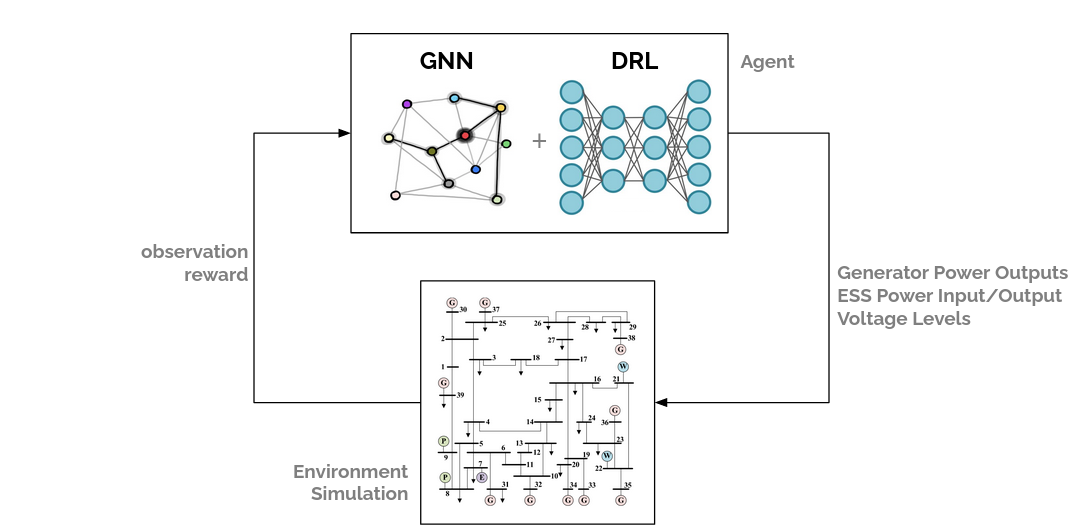
\includegraphics[width=0.85\linewidth]{./figures/arch.png}
	\caption{Solution Architecture}
	\label{fig:arch}
\end{figure}


To fulfil this, the agent adjusts the generator power output and voltage levels and manages the \ac{ESS} operation in real-time. \par
The solution is executed in the context of a power grid simulation that models the appropriate elements, properties, constraints and operating of the power distribution grid. This method is further described in the upcoming subsection \ref{sec:method}.



\section{Evaluation Metrics} \label{sec:eval-methods}

\begin{comment}
	* Sample Efficiency
	* Other methods
	* Equations
	* TODO
\end{comment}


The solution described in the previous subsections \ref{sec:arch} and \ref{sec:method} clearly involves intricate operational mechanisms, something that calls for a sophisticated evaluative process. Furthermore, given the comparative nature of this dissertation the evaluation and analysis methods will be key factors in studying and confronting the different combinations of \acp{GNN} and \ac{DRL}, as well as possible improvements in the integration of these techniques.
In this manner, we define the four dimensions for evaluating and analysing the different \ac{GRL} models:

\begin{description}
	\item[Learning efficiency] This dimension assesses how effectively the models learn and improve their decision-making process over time. It involves evaluating how quickly they converge to optimal or near-optimal dispatch strategies through the convergence rate. 
	
	\item[Computational Efficiency] It's crucial that the solution is able to perform well on real-time execution. In this context, not only it's important to assess the solution's decision computation performance but also to measure the time necessary for the model offline training, as well as the observed CPU/GPU resource utilization.
	
	\item[Dispatch Efficiency] The performance of the \ac{GRL} model in managing power distribution from the various generators will be mainly measured by the average operating cost (in \textit{Euros}) derived from the agent's sequence. Furthermore, other system behaviours will be analysed such as Renewable Energy Source Penetration, through the average ratio of maximum power and real power output, and \ac{ESS} utilization, through the average energy stored.
	
	\item[Scalability and Adaptation]  The solution will be applied to scenarios of several sizes for analysing its scalability. Furthermore, we will induce variations in the simulation scenarios to test the model's ability to handle topology changes.
\end{description}

\section{Work Plan} \label{sec:work-plan}


In order to make this project possible, we propose a 40-week work plan divided into four stages, whose start was in the last week of September 2023 and expected conclusion is scheduled for the last week of June 2024, observable in figure \ref{fig:gantt-chart}. 
The first stage, ranging from the first week of the plan to the delivery of this report, encompasses the \textbf{dissertation preparation} phase. This stage mainly addressed the initial knowledge acquisition necessary to understand this work's context and gather a basic grasp on the concepts and topics it addresses, namely:
\begin{itemize}
	 \item Reinforcement Learning
	\item Graph Theory
	\item Graph Representation Learning
	\item Graph Reinforcement Learning
	\item Graph Neural Networks
	\item Smart Grids Services
\end{itemize}
This process is followed by the analysis of existing research and approaches in \ac{GRL} and Smart Grid technologies which spans till the first week of January 2024, documented in chapter \ref{chap:literature-review}. Lastly, the preparation phase is also compromised of the PDIS report write-up until its delivery in the first week of February 2024, marking the end of this phase. \par
The preparation phase is followed by the \textbf{Development} phase. This stage encompasses all activities related to the system implementation, from the preparation of the simulation environment to the model training and calibration. The development phase spans from the first week of February 2024 to the second-to-last week of April 2024. \par
Next, the \textbf{Evaluation \& Analysis} stage is set, compromising the time frame where the various implemented models will be evaluated in the context of the previously mentioned dimensions and the evaluation results will be analysed. \par
Lastly, the \textbf{Dissertation} write-up and subsequent revision work will be performed, compromised of the write-up, proofreading and correction tasks and ranging from the end of the evaluation and analysis phase in the last week of April 2024 until the last week of the plan.


\begin{sidewaysfigure}
	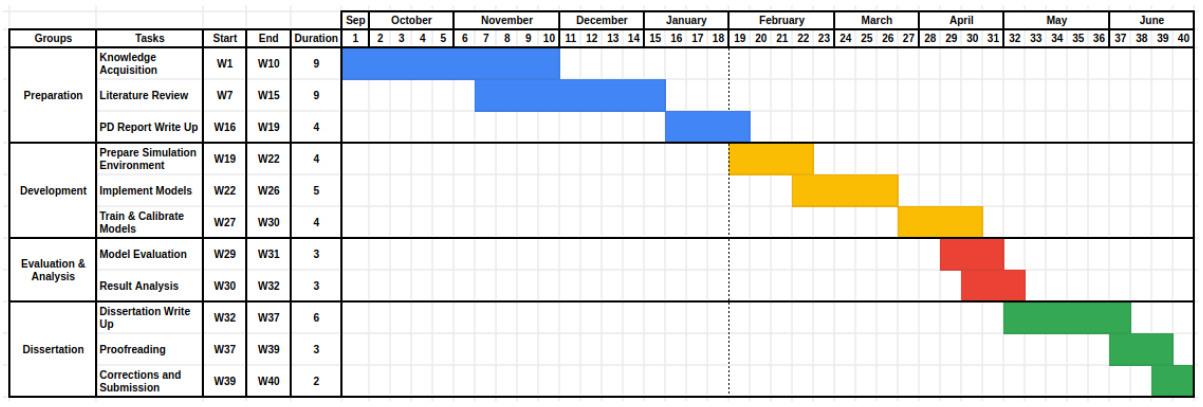
\includegraphics[width=1.0\linewidth]{./figures/gantt-chart.png}
	\caption{Project Work Plan}
	\label{fig:gantt-chart}
\end{sidewaysfigure}

